\documentclass{standalone}
\usepackage{tikz}
\usetikzlibrary{patterns, positioning}
\usepackage[sfdefault]{ClearSans} %% option 'sfdefault' activates Clear Sans as the default text font
\usepackage[T1]{fontenc}

\begin{document}
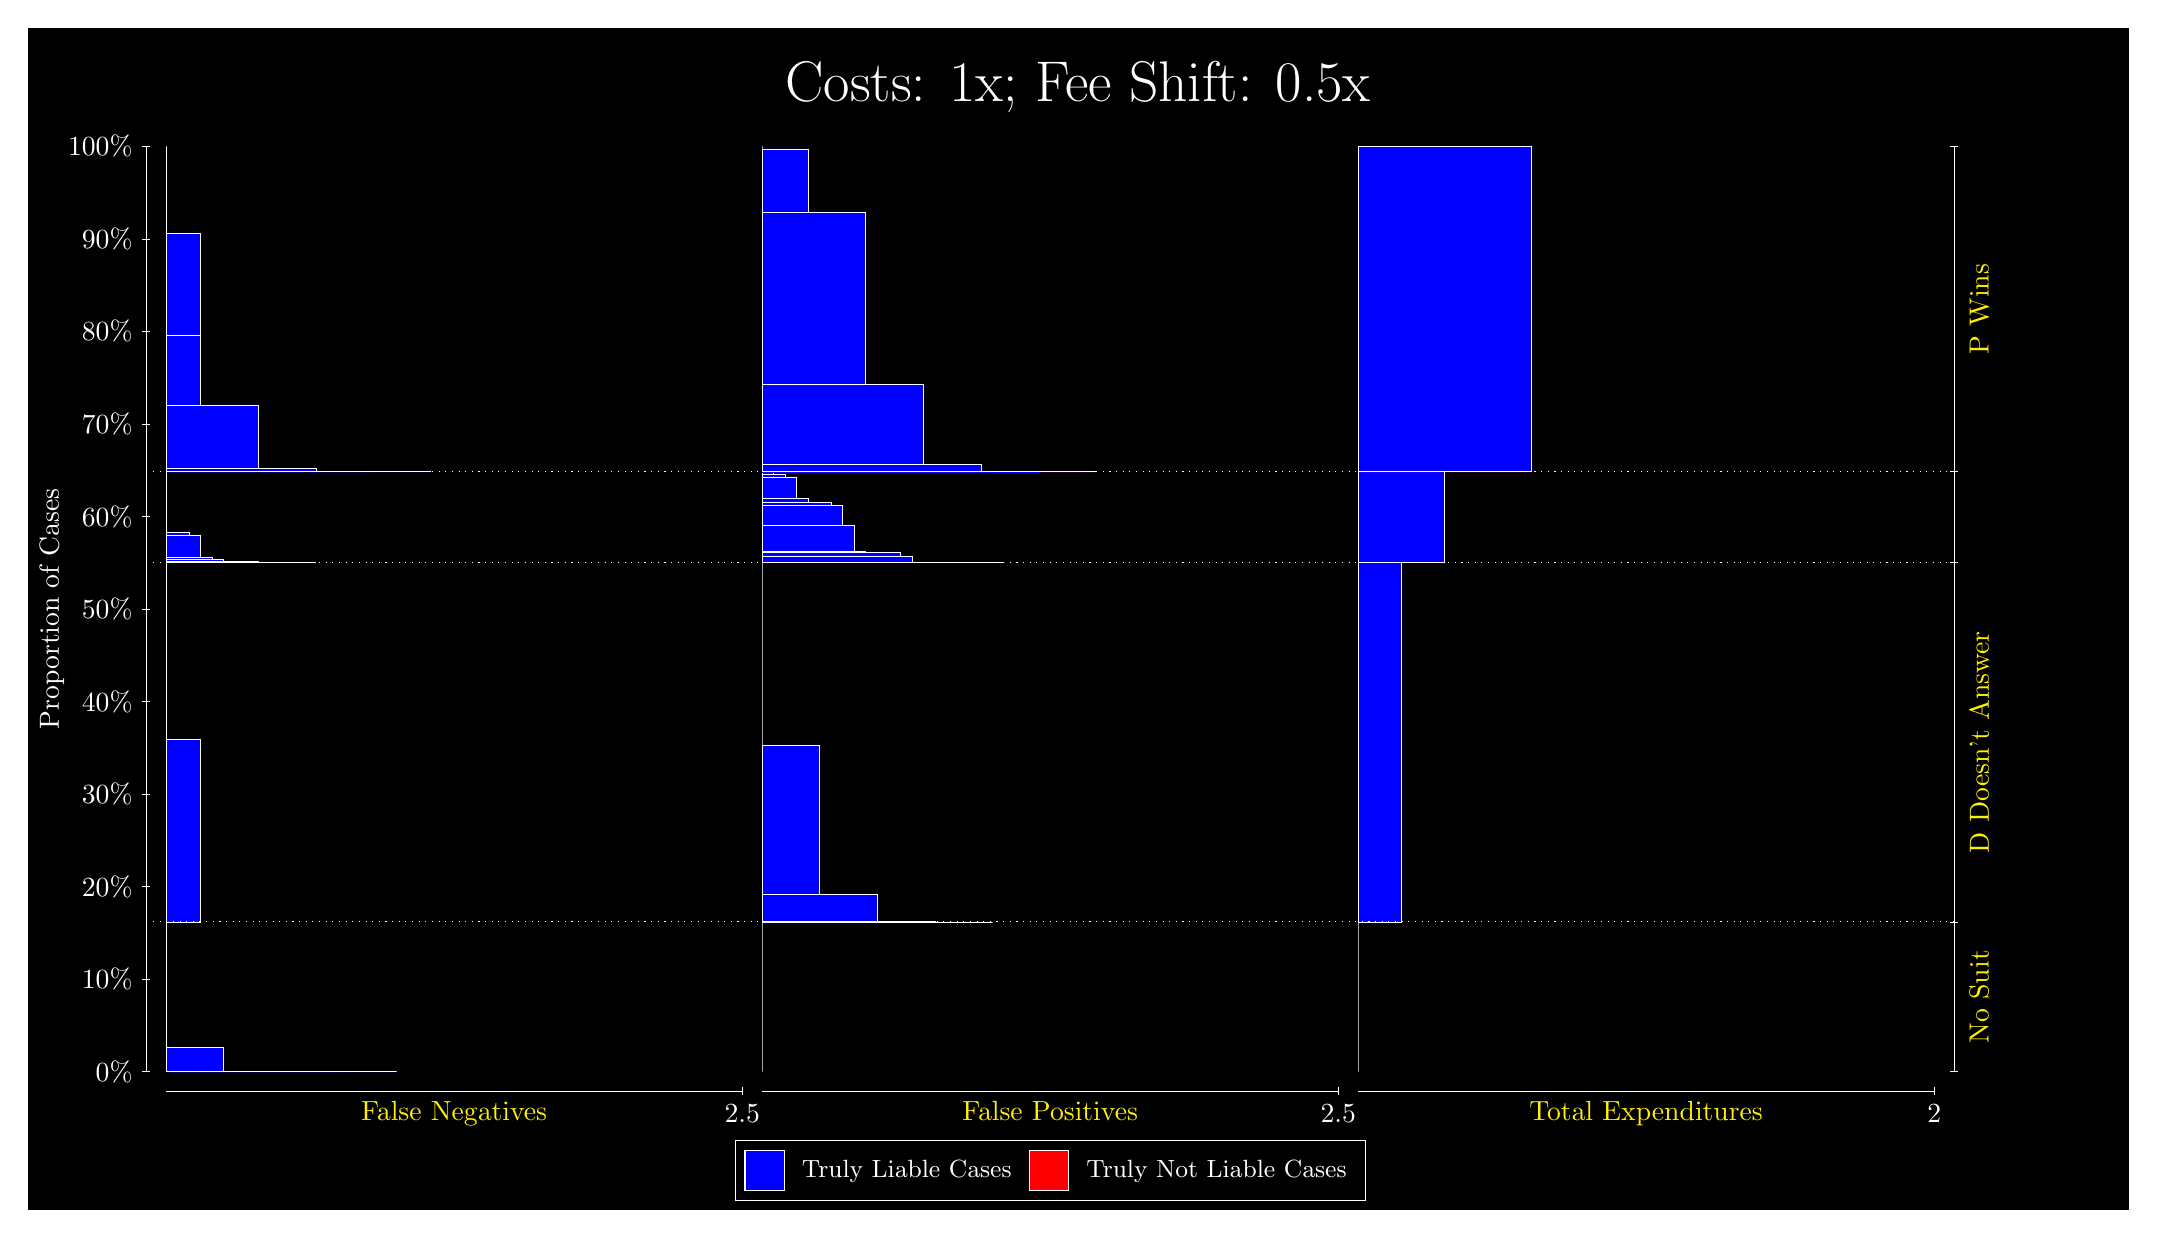
\begin{tikzpicture}
\draw[fill=black] (0,0) rectangle (26.667,15);
\draw[text=white] (0,13.5) rectangle (26.667,15) node[midway] {\huge Costs: 1x; Fee Shift: 0.5x};
\draw[white, very thin] (1.5,1.75) -- (1.5,13.5);
\node[rotate=90, text=white, anchor=center] at (0.3, 7.625) {Proportion of Cases};
\draw[white, very thin] (1.45,1.75) -- (1.55,1.75);
\node[text=white, anchor=east] at (1.45, 1.75) {0\%};
\draw[white, very thin] (1.45,2.925) -- (1.55,2.925);
\node[text=white, anchor=east] at (1.45, 2.925) {10\%};
\draw[white, very thin] (1.45,4.1) -- (1.55,4.1);
\node[text=white, anchor=east] at (1.45, 4.1) {20\%};
\draw[white, very thin] (1.45,5.275) -- (1.55,5.275);
\node[text=white, anchor=east] at (1.45, 5.275) {30\%};
\draw[white, very thin] (1.45,6.45) -- (1.55,6.45);
\node[text=white, anchor=east] at (1.45, 6.45) {40\%};
\draw[white, very thin] (1.45,7.625) -- (1.55,7.625);
\node[text=white, anchor=east] at (1.45, 7.625) {50\%};
\draw[white, very thin] (1.45,8.8) -- (1.55,8.8);
\node[text=white, anchor=east] at (1.45, 8.8) {60\%};
\draw[white, very thin] (1.45,9.975) -- (1.55,9.975);
\node[text=white, anchor=east] at (1.45, 9.975) {70\%};
\draw[white, very thin] (1.45,11.15) -- (1.55,11.15);
\node[text=white, anchor=east] at (1.45, 11.15) {80\%};
\draw[white, very thin] (1.45,12.325) -- (1.55,12.325);
\node[text=white, anchor=east] at (1.45, 12.325) {90\%};
\draw[white, very thin] (1.45,13.5) -- (1.55,13.5);
\node[text=white, anchor=east] at (1.45, 13.5) {100\%};

\draw[white, very thin] (24.457,1.75) -- (24.457,13.5);
\draw[white, very thin] (24.407,1.75) -- (24.507,1.75);
\node[anchor=west] at (24.407, 1.75) {};
\draw[white, very thin] (24.407,3.6502) -- (24.507,3.6502);
\node[anchor=west] at (24.407, 3.6502) {};
\draw[white, very thin] (24.407,8.2152) -- (24.507,8.2152);
\node[anchor=west] at (24.407, 8.2152) {};
\draw[white, very thin] (24.407,9.3678) -- (24.507,9.3678);
\node[anchor=west] at (24.407, 9.3678) {};
\draw[white, very thin] (24.407,13.5) -- (24.507,13.5);
\node[anchor=west] at (24.407, 13.5) {};

\draw[white, very thin, fill=blue] (1.75,1.75) rectangle (4.6775,1.75);
\draw[white, very thin, fill=blue] (1.75,1.75) rectangle (3.9457,1.75);
\draw[white, very thin, fill=blue] (1.75,1.75) rectangle (3.2138,1.7527);
\draw[white, very thin, fill=blue] (1.75,1.7527) rectangle (2.4819,2.0611);
\draw[white, very thin, fill=red] (1.75,2.0611) rectangle (1.75,2.0611);
\draw[white, very thin, fill=blue] (1.75,2.0611) rectangle (1.75,3.6502);
\draw[white, very thin, fill=blue] (1.75,3.6502) rectangle (2.1891,5.9722);
\draw[white, very thin, fill=red] (1.75,5.9722) rectangle (1.75,5.9722);
\draw[white, very thin, fill=blue] (1.75,5.9722) rectangle (1.75,8.2152);
\draw[white, very thin, fill=blue] (1.75,8.2152) rectangle (3.6529,8.2152);
\draw[white, very thin, fill=blue] (1.75,8.2152) rectangle (3.0674,8.2153);
\draw[white, very thin, fill=blue] (1.75,8.2153) rectangle (2.921,8.2252);
\draw[white, very thin, fill=blue] (1.75,8.2252) rectangle (2.7746,8.2275);
\draw[white, very thin, fill=blue] (1.75,8.2275) rectangle (2.4819,8.2493);
\draw[white, very thin, fill=blue] (1.75,8.2493) rectangle (2.3355,8.2809);
\draw[white, very thin, fill=blue] (1.75,8.2809) rectangle (2.1891,8.5577);
\draw[white, very thin, fill=blue] (1.75,8.5577) rectangle (2.0428,8.603);
\draw[white, very thin, fill=red] (1.75,8.603) rectangle (1.75,8.603);
\draw[white, very thin, fill=blue] (1.75,8.603) rectangle (1.75,9.3678);
\draw[white, very thin, fill=blue] (1.75,9.3678) rectangle (5.1167,9.3678);
\draw[white, very thin, fill=blue] (1.75,9.3678) rectangle (4.3848,9.3679);
\draw[white, very thin, fill=blue] (1.75,9.3679) rectangle (3.6529,9.408);
\draw[white, very thin, fill=blue] (1.75,9.408) rectangle (2.921,10.211);
\draw[white, very thin, fill=blue] (1.75,10.211) rectangle (2.1891,11.101);
\draw[white, very thin, fill=blue] (1.75,11.101) rectangle (2.1891,12.395);
\draw[white, very thin, fill=red] (1.75,12.395) rectangle (1.75,12.395);
\draw[white, very thin, fill=blue] (1.75,12.395) rectangle (1.75,13.5);
\draw[white, very thin, fill=red] (9.3189,1.75) rectangle (9.3189,1.75);
\draw[white, very thin, fill=blue] (9.3189,1.75) rectangle (9.3189,3.6502);
\draw[white, very thin, fill=red] (9.3189,3.6502) rectangle (12.246,3.6502);
\draw[white, very thin, fill=blue] (9.3189,3.6502) rectangle (12.246,3.6502);
\draw[white, very thin, fill=blue] (9.3189,3.6502) rectangle (11.515,3.6528);
\draw[white, very thin, fill=blue] (9.3189,3.6528) rectangle (10.783,4.0049);
\draw[white, very thin, fill=blue] (9.3189,4.0049) rectangle (10.051,5.8932);
\draw[white, very thin, fill=blue] (9.3189,5.8932) rectangle (9.3189,8.2152);
\draw[white, very thin, fill=red] (9.3189,8.2152) rectangle (12.393,8.2152);
\draw[white, very thin, fill=blue] (9.3189,8.2152) rectangle (12.393,8.2152);
\draw[white, very thin, fill=red] (9.3189,8.2152) rectangle (12.1,8.2152);
\draw[white, very thin, fill=blue] (9.3189,8.2152) rectangle (12.1,8.2152);
\draw[white, very thin, fill=red] (9.3189,8.2152) rectangle (11.807,8.2152);
\draw[white, very thin, fill=blue] (9.3189,8.2152) rectangle (11.807,8.2153);
\draw[white, very thin, fill=blue] (9.3189,8.2153) rectangle (11.661,8.2153);
\draw[white, very thin, fill=blue] (9.3189,8.2153) rectangle (11.368,8.2155);
\draw[white, very thin, fill=red] (9.3189,8.2155) rectangle (11.222,8.2155);
\draw[white, very thin, fill=blue] (9.3189,8.2155) rectangle (11.222,8.2893);
\draw[white, very thin, fill=blue] (9.3189,8.2893) rectangle (11.075,8.3413);
\draw[white, very thin, fill=blue] (9.3189,8.3413) rectangle (10.929,8.3429);
\draw[white, very thin, fill=blue] (9.3189,8.3429) rectangle (10.636,8.3616);
\draw[white, very thin, fill=blue] (9.3189,8.3616) rectangle (10.49,8.6906);
\draw[white, very thin, fill=blue] (9.3189,8.6906) rectangle (10.344,8.9369);
\draw[white, very thin, fill=blue] (9.3189,8.9369) rectangle (10.197,8.98);
\draw[white, very thin, fill=blue] (9.3189,8.98) rectangle (9.9044,9.0253);
\draw[white, very thin, fill=blue] (9.3189,9.0253) rectangle (9.758,9.3021);
\draw[white, very thin, fill=blue] (9.3189,9.3021) rectangle (9.6116,9.3337);
\draw[white, very thin, fill=blue] (9.3189,9.3337) rectangle (9.4652,9.3555);
\draw[white, very thin, fill=blue] (9.3189,9.3555) rectangle (9.3189,9.3678);
\draw[white, very thin, fill=red] (9.3189,9.3678) rectangle (13.564,9.3678);
\draw[white, very thin, fill=blue] (9.3189,9.3678) rectangle (13.564,9.3678);
\draw[white, very thin, fill=red] (9.3189,9.3678) rectangle (12.832,9.3678);
\draw[white, very thin, fill=blue] (9.3189,9.3678) rectangle (12.832,9.3689);
\draw[white, very thin, fill=red] (9.3189,9.3689) rectangle (12.1,9.3689);
\draw[white, very thin, fill=blue] (9.3189,9.3689) rectangle (12.1,9.4597);
\draw[white, very thin, fill=red] (9.3189,9.4597) rectangle (11.368,9.4597);
\draw[white, very thin, fill=blue] (9.3189,9.4597) rectangle (11.368,10.472);
\draw[white, very thin, fill=red] (9.3189,10.472) rectangle (10.636,10.472);
\draw[white, very thin, fill=blue] (9.3189,10.472) rectangle (10.636,12.657);
\draw[white, very thin, fill=blue] (9.3189,12.657) rectangle (9.9044,13.46);
\draw[white, very thin, fill=blue] (9.3189,13.46) rectangle (9.3189,13.5);
\draw[white, very thin, fill=red] (16.888,1.75) rectangle (16.888,1.75);
\draw[white, very thin, fill=blue] (16.888,1.75) rectangle (16.888,3.6502);
\draw[white, very thin, fill=red] (16.888,3.6502) rectangle (17.437,3.6502);
\draw[white, very thin, fill=blue] (16.888,3.6502) rectangle (17.437,8.2152);
\draw[white, very thin, fill=red] (16.888,8.2152) rectangle (17.986,8.2152);
\draw[white, very thin, fill=blue] (16.888,8.2152) rectangle (17.986,9.3678);
\draw[white, very thin, fill=red] (16.888,9.3678) rectangle (19.083,9.3678);
\draw[white, very thin, fill=blue] (16.888,9.3678) rectangle (19.083,13.5);
\draw[white, dotted] (1.5,3.6502) -- (24.457,3.6502);
\draw[white, dotted] (1.5,8.2152) -- (24.457,8.2152);
\draw[white, dotted] (1.5,9.3678) -- (24.457,9.3678);
\draw[white, very thin] (1.75,1.5) -- (9.0689,1.5);
\node[text=yellow, anchor=north] at (5.4094, 1.5) {False Negatives};
\draw[white, very thin] (9.0689,1.45) -- (9.0689,1.55);
\node[text=white, anchor=north] at (9.0689, 1.45) {2.5};

\draw[white, very thin] (9.3189,1.5) -- (16.638,1.5);
\node[text=yellow, anchor=north] at (12.978, 1.5) {False Positives};
\draw[white, very thin] (16.638,1.45) -- (16.638,1.55);
\node[text=white, anchor=north] at (16.638, 1.45) {2.5};

\draw[white, very thin] (16.888,1.5) -- (24.207,1.5);
\node[text=yellow, anchor=north] at (20.547, 1.5) {Total Expenditures};
\draw[white, very thin] (24.207,1.45) -- (24.207,1.55);
\node[text=white, anchor=north] at (24.207, 1.45) {2};

\node[text=yellow, centered, rotate=90] at (24.777, 2.7001) {No Suit};
\node[text=yellow, centered, rotate=90] at (24.777, 5.9327) {D Doesn't Answer};

\node[text=yellow, centered, rotate=90] at (24.777, 11.434) {P Wins};

\draw (12.978300999999998,1.5) node[draw=none] (baseCoordinate) {};
\begin{scope}[align=center]
        \matrix[scale=0.5, draw=white, below=0.5cm of baseCoordinate, nodes={draw}, column sep=0.1cm]{
            \node[rectangle, draw, minimum width=0.5cm, minimum height=0.5cm, fill=blue] {}; &
            \node[draw=none, font=\small, text=white] (B) {Truly Liable Cases}; &
            \node[rectangle, draw, minimum width=0.5cm, minimum height=0.5cm, fill=red] {}; &
            \node[draw=none, font=\small, text=white] (B) {Truly Not Liable Cases}; \\
            };
\end{scope}

\end{tikzpicture}
\end{document}